\documentclass{article}
\usepackage[margin=.75in]{geometry}
\usepackage{graphicx, dblfloatfix}
\usepackage{amsmath, amssymb, amsfonts, mathrsfs, mathtools}
\usepackage[english]{babel}
\usepackage[autostyle, english = american]{csquotes}
\MakeOuterQuote{"}

\newcommand{\redchi}{$\tilde{\chi}^2\,$}
\DeclareMathOperator{\erf}{erf}
\DeclareMathOperator{\cov}{cov}
\newcommand{\dipole}{$\vec{\mu}\,$}
\newcommand{\B}{$\vec{B}\,$}
\newcommand{\E}{$\vec{E}\,$}
\DeclarePairedDelimiter\abs{\lvert}{\rvert}%

\title{Electron Spin Resonance}
\author{Aman LaChapelle}

\begin{document}
\raggedright
\maketitle

\begin{abstract}
	The classical example of a magnetic dipole moment reacting in a magnetic field is the electron.  Here we will investigate the reaction of a particle with a dipole moment in a magnetic field and investigate how it changes in analogy to the elctron.  We begin with a classical analogue of the electron and move on to an ensemble of electrons.  These electrons are bound in DPPH, rather than being a 3D gas, but for all intents and purposes will serve to illustrate the properties we are investigating here.
\end{abstract}

\tableofcontents
\newpage

\section{Introduction}
	The magnetic dipole moment of a charged particle is related to the spin of the particle in the simple analogue of a current loop.  Charges going around a closed loop have a magnetic dipole moment
	\begin{equation*}
		\vec{\mu} = IA\hat{n}
	\end{equation*}
	with $\hat{n}$ being the unit vector normal to the area $A$.  This generates a magnetic dipole field, equal to
	\begin{equation*}
		B = \frac{\mu_0}{4\pi}\bigg{(}\frac{3r(\vec{\mu} \cdot \vec{r})}{r^5} - \frac{\mu}{r^3}\bigg{)}.
	\end{equation*}

	This assumes no external field, however.  If there is an external field, and \dipole is not perfectly aligned, we will see precession about the external field (assuming a DC field pointing in one direction).  We can measure this property both in our classical analogue to an electron, and in actual electrons.  This effect is also very important in other physics.  For example, in microwave resonators we use crystals of Yttrium-Iron-Garnet which have the property that an AC \B field of approximately 2000 Gauss will cause them to precess at microwave frequency in such a way that couples strongly to the resonator.  This has many useful applications, and there is some extremely interesting physics we can study simply by looking at the precession of the magnetic dipole moment.



\section{Theory}
	We can derive the precession about the external field beginning with the torque felt by \dipole when placed in an external field.  We will begin with the Maxwell Stress Tensor.  In the case of a dipole moment that is not aligned to the external field, we see that the stress tensor is asymmetric.  Since the stress tensor is given (in this case - neglecting the small \E fields) by
	\begin{equation*}
		\sigma_{ij} = \frac{H_iH_j}{4\pi} - \frac{H^2}{8\pi}\delta_{ij}
	\end{equation*}
	for situations in vacuum.  We realize from this equation that if two fields are not colinear then the tensor will be asymmetric.  In order to recover the symmetry (and minimize the energy by aligning the fields), there will be some torque on the object.  Furthermore, since we are interested in the magnetic dipole moment let us recognize that
	\begin{equation*}
		H = \frac{B}{\mu_0} - \int_{V}\vec{\mu}\,dV.
	\end{equation*}
	Thus we can write
	\begin{gather*}
		\tau_i = -\epsilon_{ijk}\sigma_{jk}\\
		\tau_i = -\epsilon_{ijk}\frac{H_jB_k}{4\pi}\\
		\vec{\tau} = \frac{-\vec{H} \times \vec{B}}{4\pi}
	\end{gather*}
	\begin{equation}
		\vec{\tau} = \vec{\mu} \times \vec{B}
	\end{equation}

	Now that we know the torque exerted on the magnetic moment by the external field, we can begin to work through the precession and the frequency of precession caused by that torque.

	\begin{figure}[!htb]
		\centering
		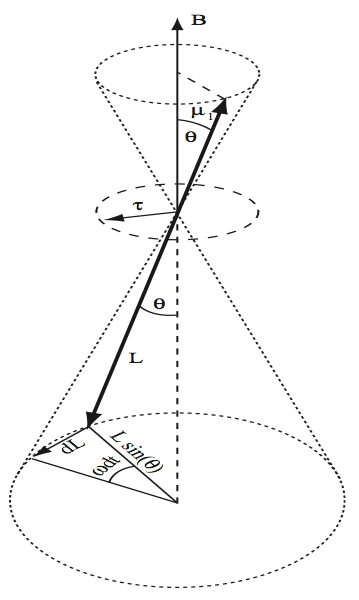
\includegraphics[scale=.5]{../figures/torque}
		\caption{The precession of \dipole about an external \B field.}
	\end{figure}

	Figure 1 provides us with some intuition into how to go about finding the frequency of precession of the dipole moment.  Since we can transform into a rotating frame to describe the motion of $\vec{L}$, we can write
	\begin{gather*}
		\frac{d\vec{L}}{dt} = \vec{\tau} = \vec{\omega} \times \vec{L}\\
		\vec{\mu} \times \vec{B} = \vec{\omega} \times \vec{L}
	\end{gather*}
	and since the angle between \dipole and \B is the same as the angle between $\vec{\omega}$ and $\vec{L}$ by definition of our frame, we can write 
	\begin{gather}
		\omega = \frac{\mu}{L}B\\
		\omega = \gamma B
	\end{gather}
	where $\gamma$ is the gyromagnetic ratio.  For an electron, we can express it as
	\begin{equation}
		\abs{\gamma_e} = \frac{\abs{-e}}{2m_e}g_e = \frac{g_e \mu_B}{\hbar}
	\end{equation}
	where $\mu_B$ is the Bohr Magneton and $g_e$ is given by
	\begin{equation*}
		g_e = 2\bigg{(}1+\frac{\alpha}{2\pi} + ...\bigg{)}.
	\end{equation*}

\section{Apparatus}

\section{Data Analysis}

\section{Error Analysis}

\section{Conclusion}

\begin{thebibliography}{10}
	\bibitem{first}
	stuff here\\
\end{thebibliography}

\end{document}